\chapter{CMS Experiment}

\section{Large Hadron Collider (LHC)}

The Large Hadron Collider is the largest and most powerful particle accelerator ever built. It boost protons, to produce two beams travelling in opposite directions, which collide at four points where the two rings of the machine intersect. The design energy per proton beam is of 7 TeV. The protons of the LHC circulate around the ring in well defined bunches. In the LHC, under nominal operating conditions, each proton beam has 2808 bunches, with each bunch containing about 10$^{11}$ protons. They measure a few centimetres long and a millimetre wide when they are far from a collision point. As they approach the collision points, they are squeezed to about 16 $\mu$m to allow for a greater chance of proton-proton collisions. The LHC uses a bunch spacing of 25 ns (or about 7 m), which  corresponds to a frequency of 40 MHz \cite{Bruning:2004ej}. Nowdays, each proton beam flying around the LHC have an energy of 6.5 TeV, so when two protons collide the collision energy is 13 TeV. There are seven experiments installed at the LHC (Fig. \ref{fig:LHC}); The biggest experiments consist in two general-purpose detectors to investigate the largest range of physics possible : The Compact Muon Solenoid (CMS) and A Toroidal LHC ApparatuS (ATLAS), and two specialized for focussing on specific phenomena: A Large Ion Collider Experiment (ALICE) and Large Hadron Collider beauty experiment(LHCb). The smaller experiments on the LHC are the TOTal Elastic and diffractive cross section Measurement (TOTEM), Large Hadron Collider forward experiment (LHCf) and the Monopole and Exotics Detector at the LHC (MOEDAL). The first two experiments are  focused on "forward particles", protons or heavy ions that brush past each other rather than meeting head on when the beams collide and the last experiment searches for a hypothetical particle called the magnetic monopole. TOTEM will be installed close to the CMS interaction point, LHCf will be installed near ATLAS and MOEDAL near LHCb. 

\begin{figure}[H]
\caption{The CERN accelerator complex.\label{fig:LHC}}
  \centering
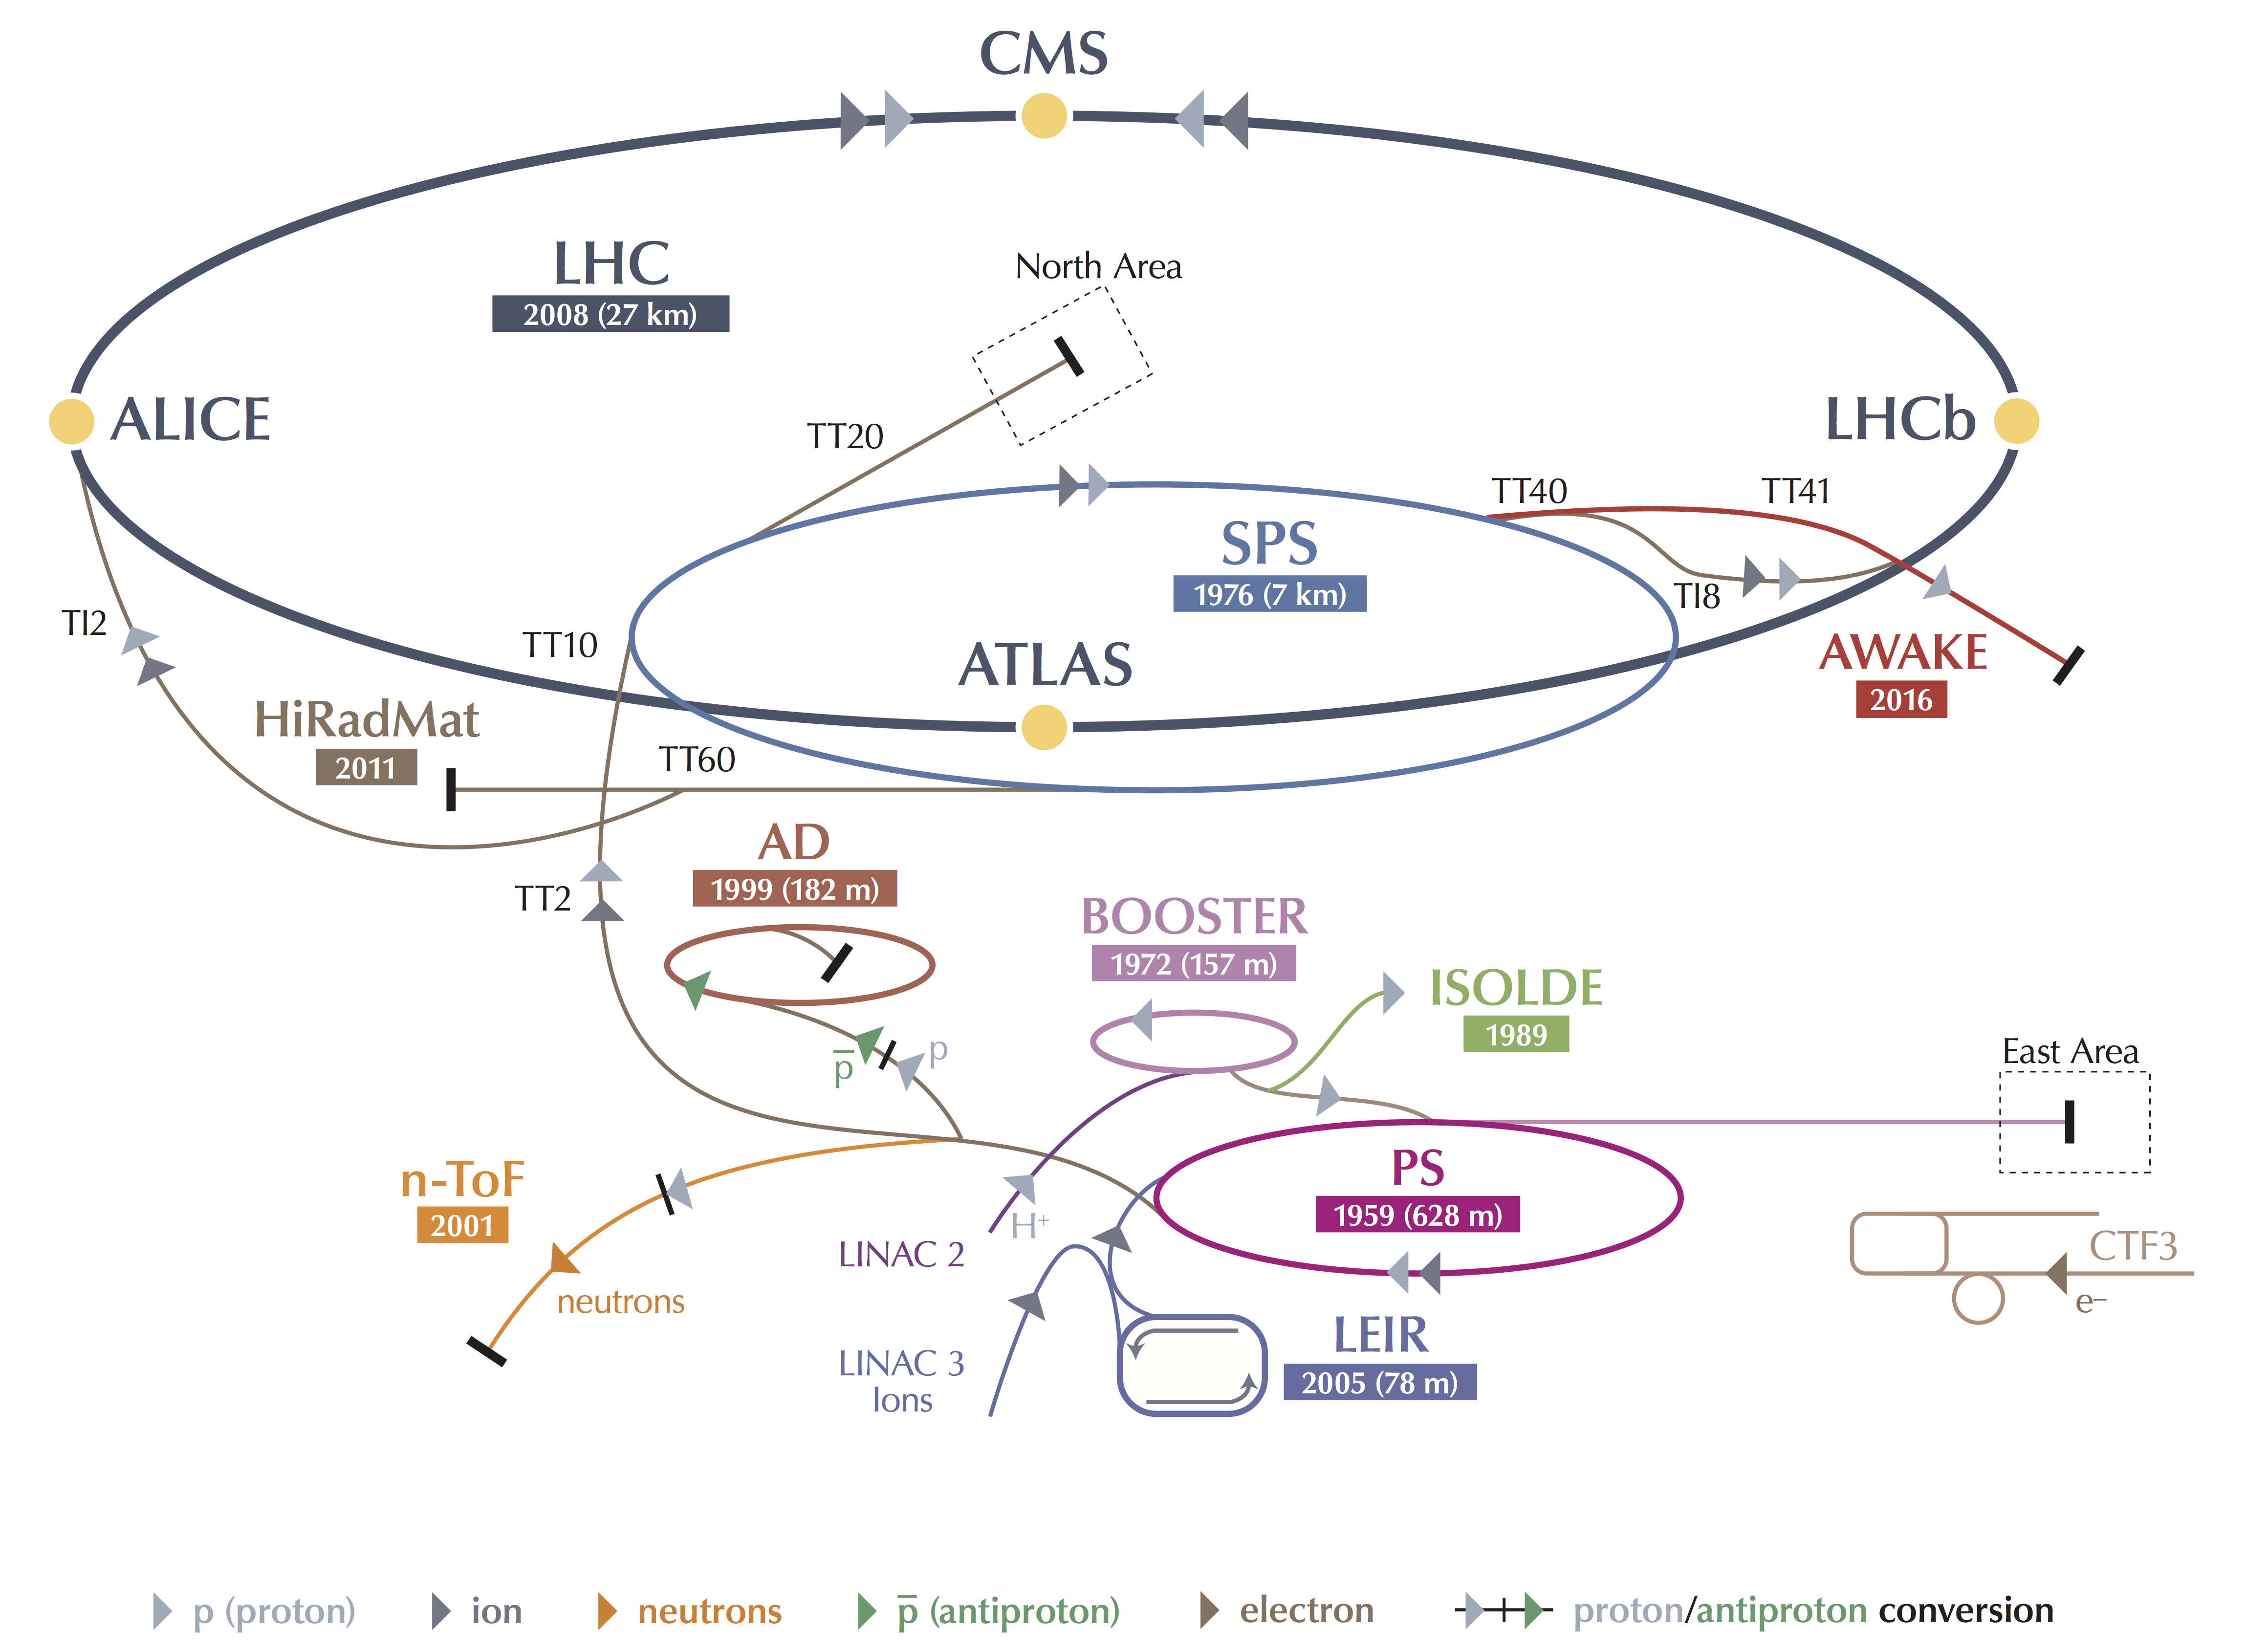
\includegraphics[width=13cm]{CMS_chapter_plots/lhc3}
\caption*{Source: The CERN accelerator complex. \cite{Haffner:1621894} }
\end{figure}

\section{CMS Detector}

The central feature of the CMS apparatus is a superconducting solenoid of \unit[6]{m} internal diameter, providing a magnetic field of \unit[3.8]{T}.Within the superconducting solenoid volume are a silicon pixel and strip tracker, a lead tungstate crystal electromagnetic calorimeter (ECAL), and a brass and scintillator hadron calorimeter (HCAL), each composed of a barrel and two endcap sections. Muons are measured in gas-ionization detectors embedded in the steel flux-return yoke outside the solenoid. Extensive forward calorimetry complements the coverage provided by the barrel and endcap detectors. A right-handed coordinate system is used with its origin at the nominal interaction point (IP). The x-axis points to the center of the LHC ring, the y-axis is vertical and points upward, and the z-axis is parallel to the counterclock-wise beam direction. The azimuthal angle $\phi$ is measured with respect to the x-axis in the xy-plane and the polar angle $\theta$ is defined with respect to the z-axis, while the pseudorapidity is defined as $\eta = -\ln\left[\tan\left(\theta/2 \right)  \right]$. Figure \ref{figure:CMS} shows an schematic view of the CMS detector and figure \ref{figure:eta} shows the $\eta$ and $\phi$ coordinates in the CMS detector.

\begin{figure}[h]
\caption{Schematic view of the CMS detector \label{figure:CMS}}
  \centering
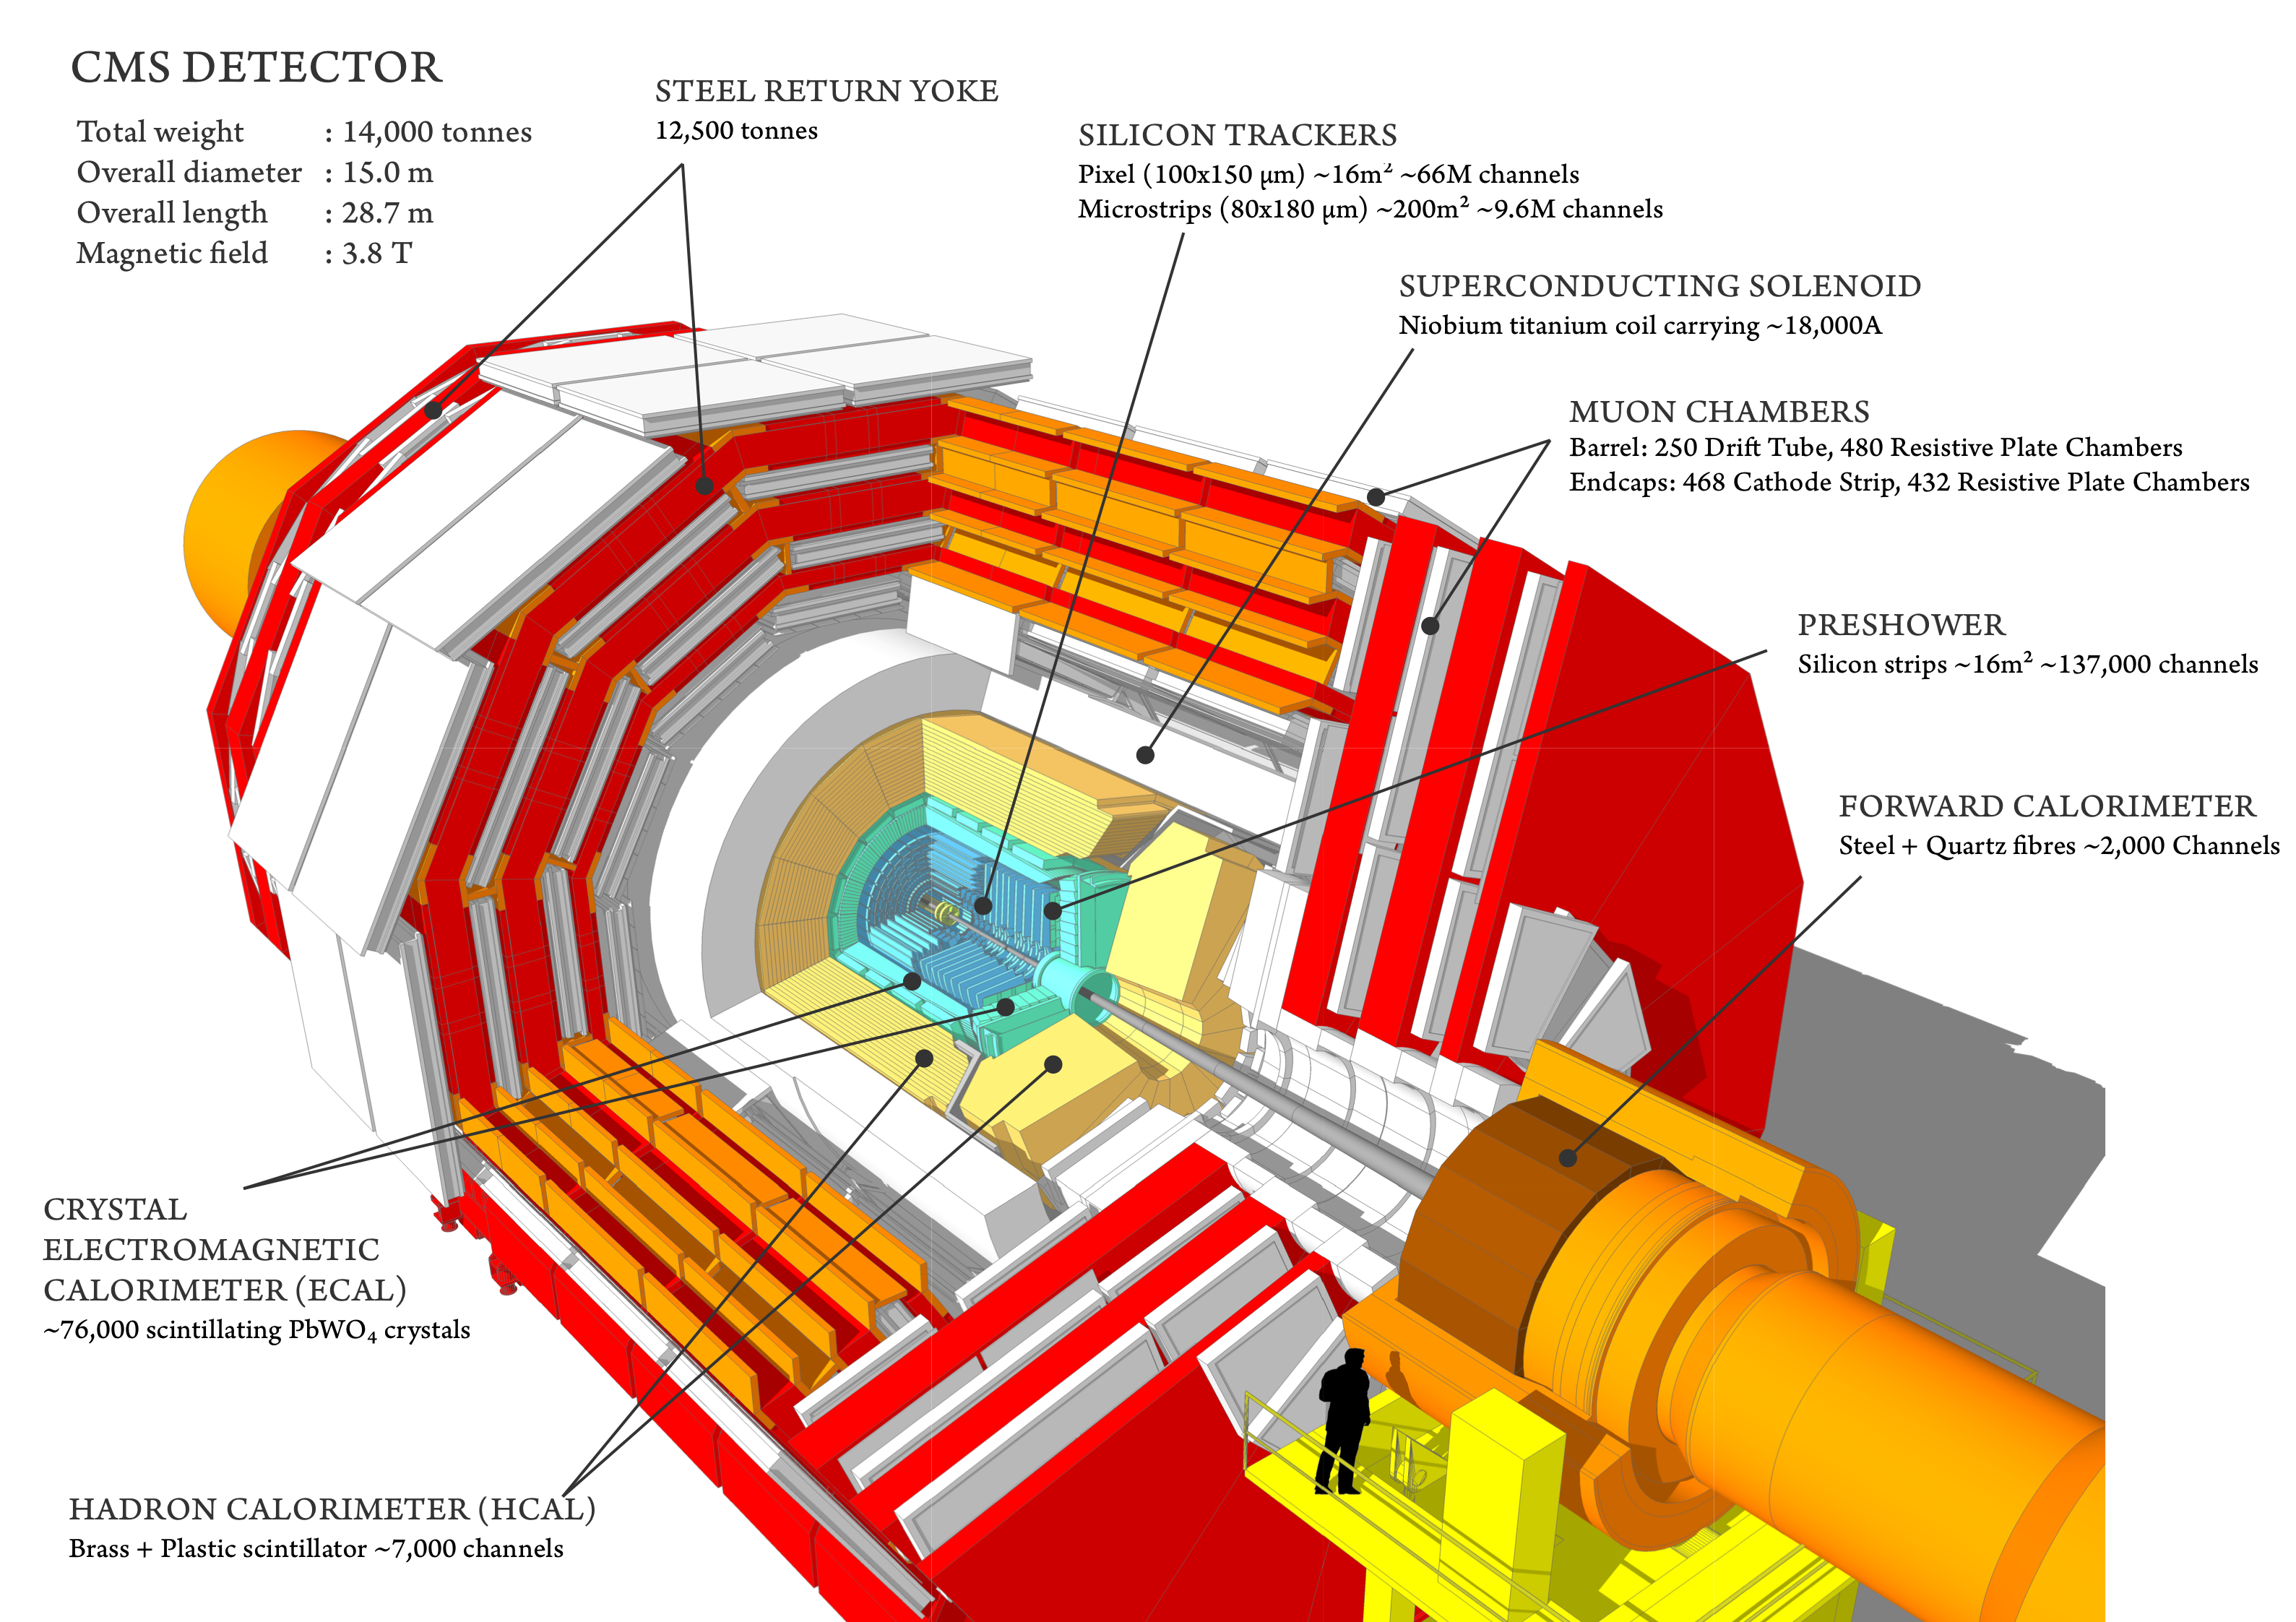
\includegraphics[width=12cm]{CMS_chapter_plots/cms_120918_03}
\caption*{Source: Detector and Event Visualization with SketchUp at the
                        CMS Experiment \cite{Sakuma:2013jqa}.}
\end{figure}

\begin{figure}[H]
\caption{$\eta$ and $\phi$ coordinates in the CMS detector. \label{figure:eta}}
  \centering
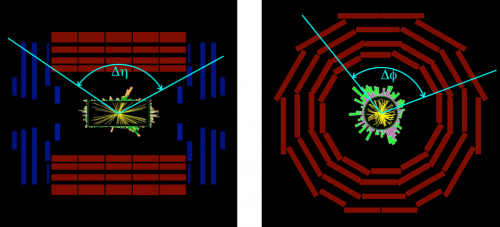
\includegraphics[width=11cm]{CMS_chapter_plots/image_eta}
\end{figure}

\subsection{The Magnet}

The CMS detector contains a 3.8 T superconducting solenoid (which produce an axial field) with a free bore of a diameter of 6 m and a length of 12.5 m, enclosed inside a 12 000 t yoke made of common structural steel. The inner diameter of the coil is large enough to set up the tracking system and the full calorimetry. Due to the number of ampere-turns required for generating a field of 3.8 T, the winding in the coil is composed of 5 modules, with four layers of conductor each. The coil is indirectly cooled by saturated helium at 4.5 K circulating in the thermosiphon mode through a network of pipes welded to the external mandrels \cite{Acquistapace:1997fm}. Figure \ref{fig:coil} shows an artistic view of the superconducting solenoid. The yoke is composed of five three-layered dodecagonal barrel wheels and three endcap disks at each end. In the barrel region the innermost yoke layer is 295 mm thick and each of the two outermost ones is 630 mm thick. The yoke contributes to only 8$\%$ of the central magnetic flux density; its main role is to increase the field homogeneity in the tracker volume and to reduce the stray field by returning
the magnetic flux of the solenoid. The demand for good momentum resolution, without making tight requests on the spatial resolution of the muon chambers, influence to the choice of a high solenoidal magnetic field. Since the magnet is the main component of CMS in terms of size, weight and structural rigidity, it is used as the principal structural element to support all barrel detector components. Figure \ref{fig:yoke} shows an schematic view of the CMS detector and their magnet components.

\begin{figure}[H]
\caption{General artistic view of the 5 modules composing the superconductiong coil. \label{fig:coil}}
  \centering
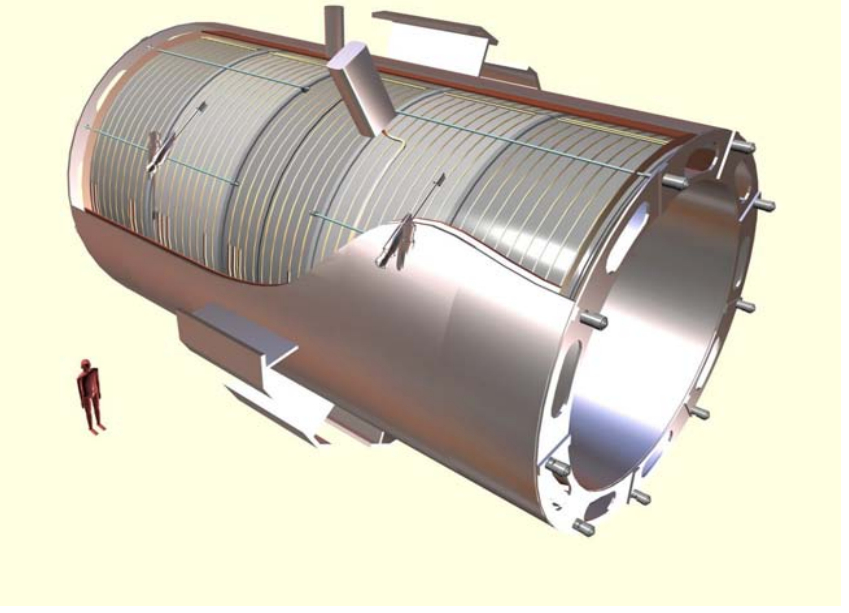
\includegraphics[width=10cm]{CMS_chapter_plots/coil}
\caption*{Source: The CMS experiment at the CERN LHC \cite{1748-0221-3-08-S08004}.}
\end{figure}

\begin{figure}[H]
\caption{Schematic views of the CMS detector, with the numbering convention for azimuthal sectors (S),
wheels (W), barrel yoke layers (L) and endcap disks (D). Left: transverse view at z = 0. Right: longitudinal view of one quarter of the detector. \label{fig:yoke}}
  \centering
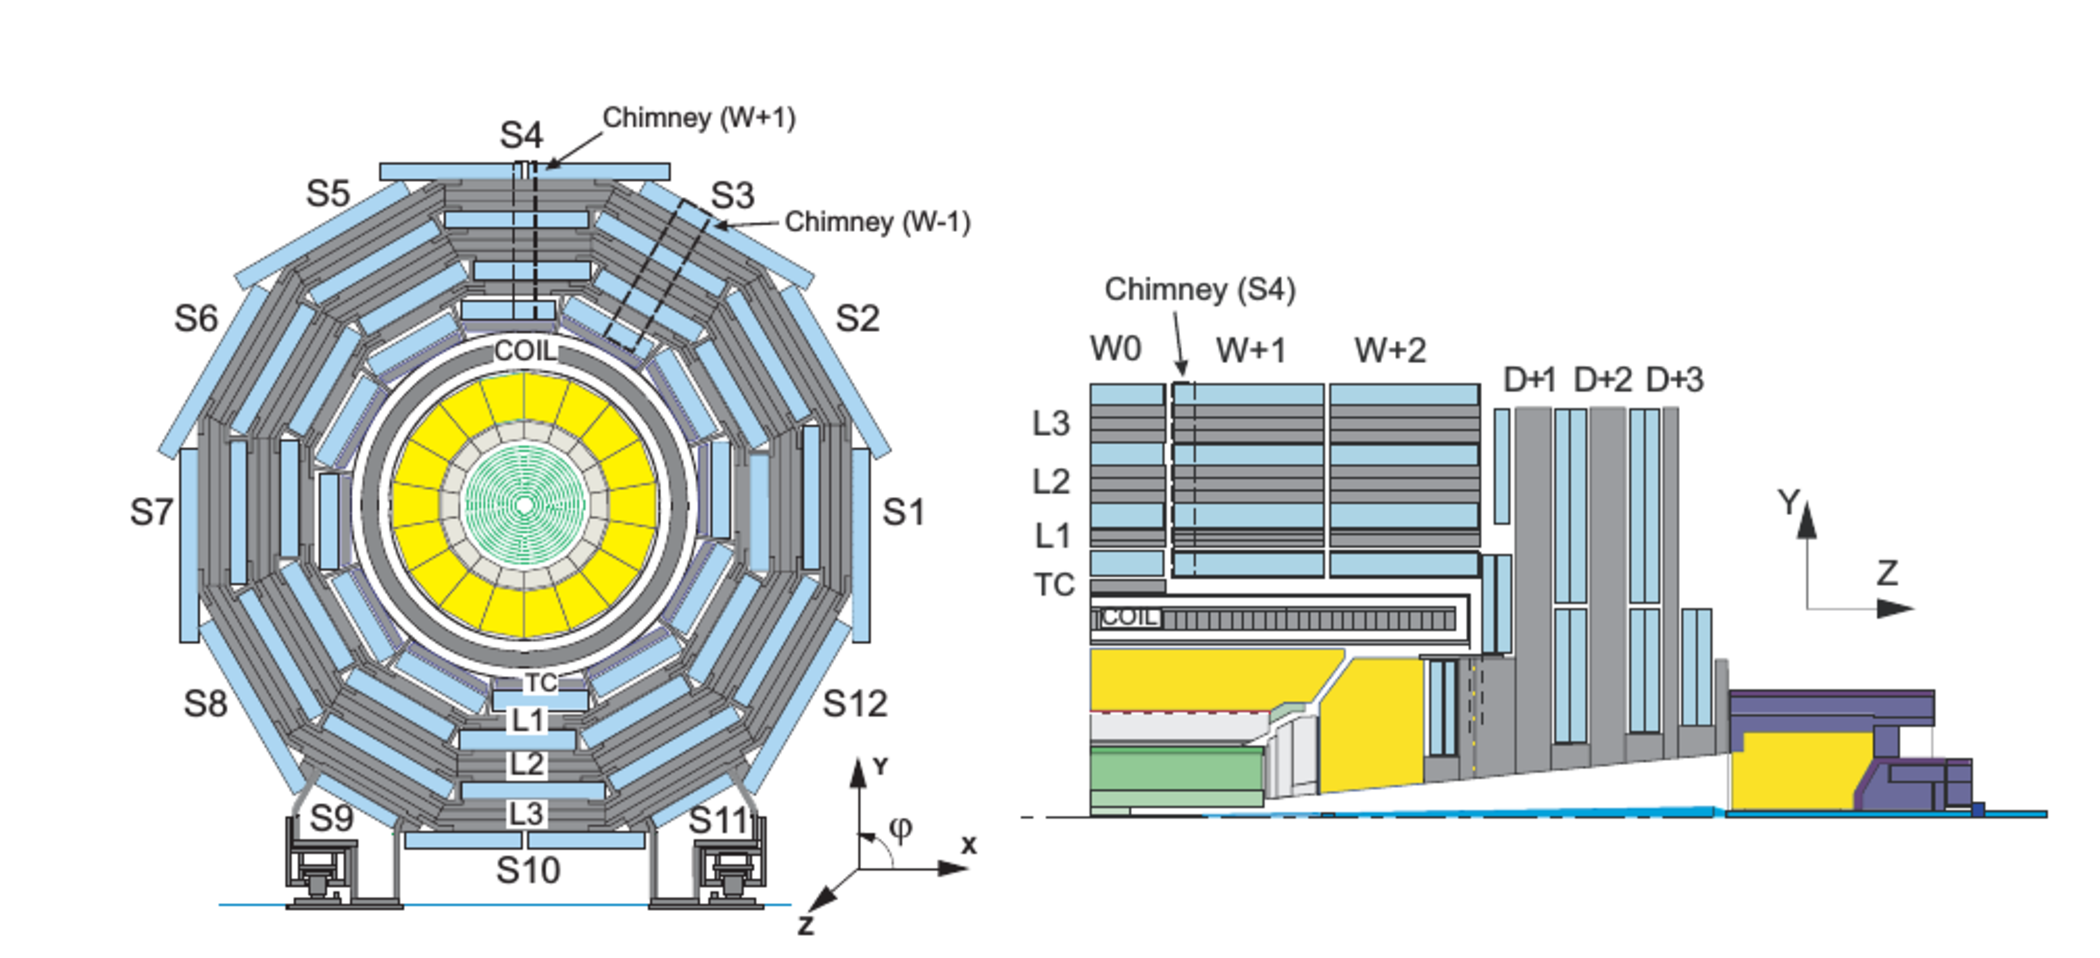
\includegraphics[width=15cm]{CMS_chapter_plots/yoke}
\caption*{Source: Precise mapping of the magnetic field in the CMS barrel yoke using cosmic rays \cite{1748-0221-5-03-T03021}.}
\end{figure}

Simulation and reconstruction of events in the CMS detector require knowledge of the magnetic
field in the entire detector, both in the inner tracking region and in the complex configuration of the
steel return yoke. Figure \ref{fig:mapas12} shows the predicted magnetic flux density on a longitudinal section of the CMS detector.

\begin{figure}[H]
\caption{Value of $\arrowvert \vec{B} \arrowvert$ (left) and field lines (right) predicted on a longitudinal section of the CMS detector, at a central magnetic flux density of 3.8 T. \label{fig:mapas12}  }
  \centering
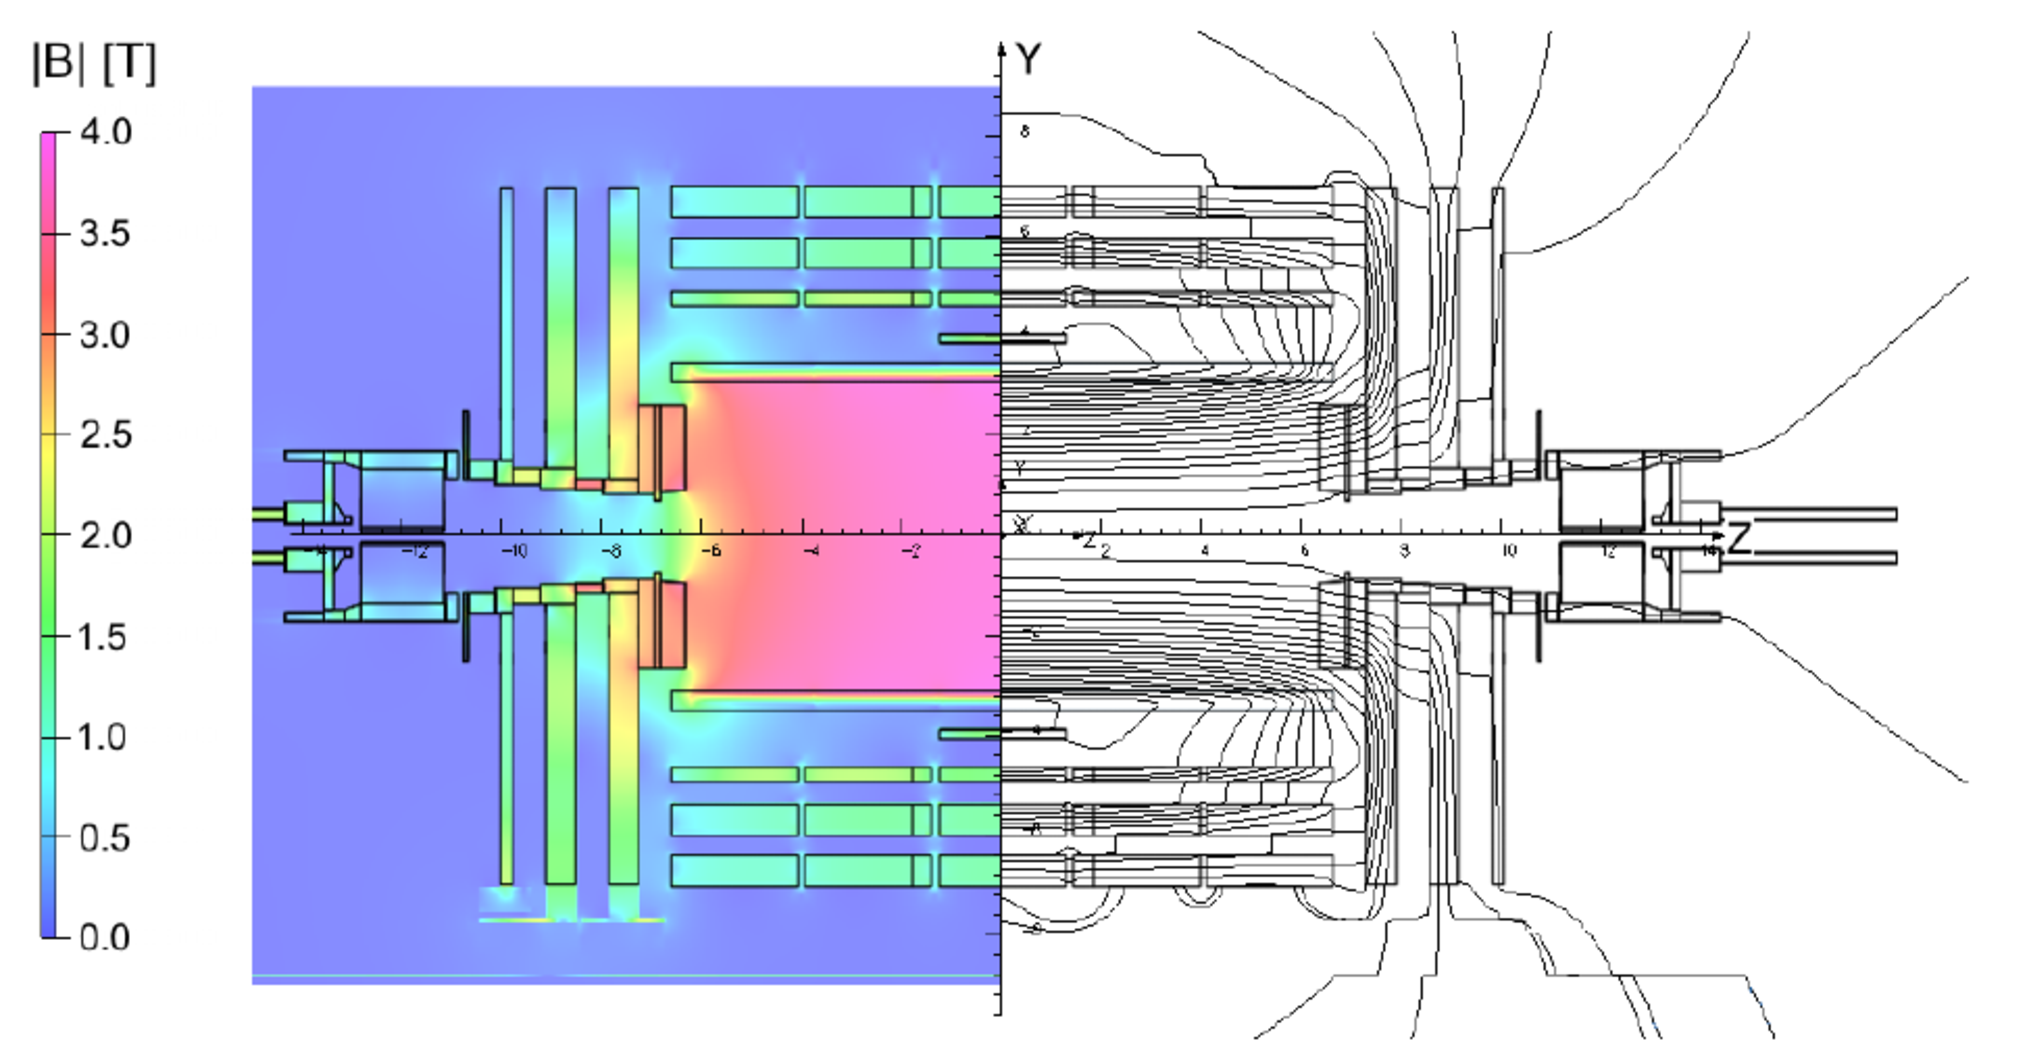
\includegraphics[width=14cm]{CMS_chapter_plots/map}
\caption*{Source: Precise mapping of the magnetic field in the CMS barrel yoke using cosmic rays \cite{1748-0221-5-03-T03021}.}
\end{figure}


\subsection{CMS Tracking system}

The main idea behind "tracking" is to measure the momentum of the particles. The hole tracking system is enclosed in a huge solenoid magnet, which produces an approximately uniform magnetic field pointing along the direction on the LHC beam. As the charged particle flies from the center of the detector, its trajectory are bended. Along its path, it leaves hits in the detecting material. In a process called track reconstruction, CMS software connects the hits and produces a track. From the information of the charge of the particle, the intensity of the magnetic field and the radius of the path, it can determine the transverse momentum of the particle. The tracking system is divide into two different subsystems, the Silicon Pixels and the Silicon Strips.

\subsubsection{Silicon pixels} \label{pixel}

The pixel tracker allows the reconstruction of charged particle trajectories in the region closest
to the interaction point. It contributes precise tracking points in $r-\phi$ and $z$ and therefore is responsible for a small impact parameter resolution that is important for good secondary vertex reconstruction \cite{1748-0221-3-08-S08004}.
The CMS pixel detector consists of about 65 million distinct pixels of 100 $\times$ 150 $\mu$m$^{2}$ spread over three cylinders of a meter long and in radius of \unit[4]{cm}, \unit[7]{cm} and \unit[10]{cm} (\cref{fig:pixel}).
When a particle passes through our silicon detector, it produce a electron-hole pairs. These electron-hole pairs are pulled in opposite directions by an electric field, and pulled into "contacts". Then, the charge built up on those contacts produces a current that flows into our electronics. The key feature of a pixel detector is that the individual contacts are two-dimensional; for every 0.05 by 0.4 millimeter pixel, there is a separate circuit and separate electronics. This gives us a very precise measurement of where, exactly, the particle passed through the detector.

\begin{figure}[H]
  \caption{Left: Sktech of the CMS pixel detector. Right: Quarter of a slice of the CMS pixel detector by a plane which contains its axis of symmetry. The centre of the detector is at the left-bottom corner of the drawing, in the interaction region. The horizontal axis, to which the detector has a cylindrical symmetry, is parallel to the LHC beams. The vertical axis points along the radius. Various pseudo-rapidity values are shown at the ends of the black dashed lines. \label{fig:pixel}}
\begin{tabular}{cc}
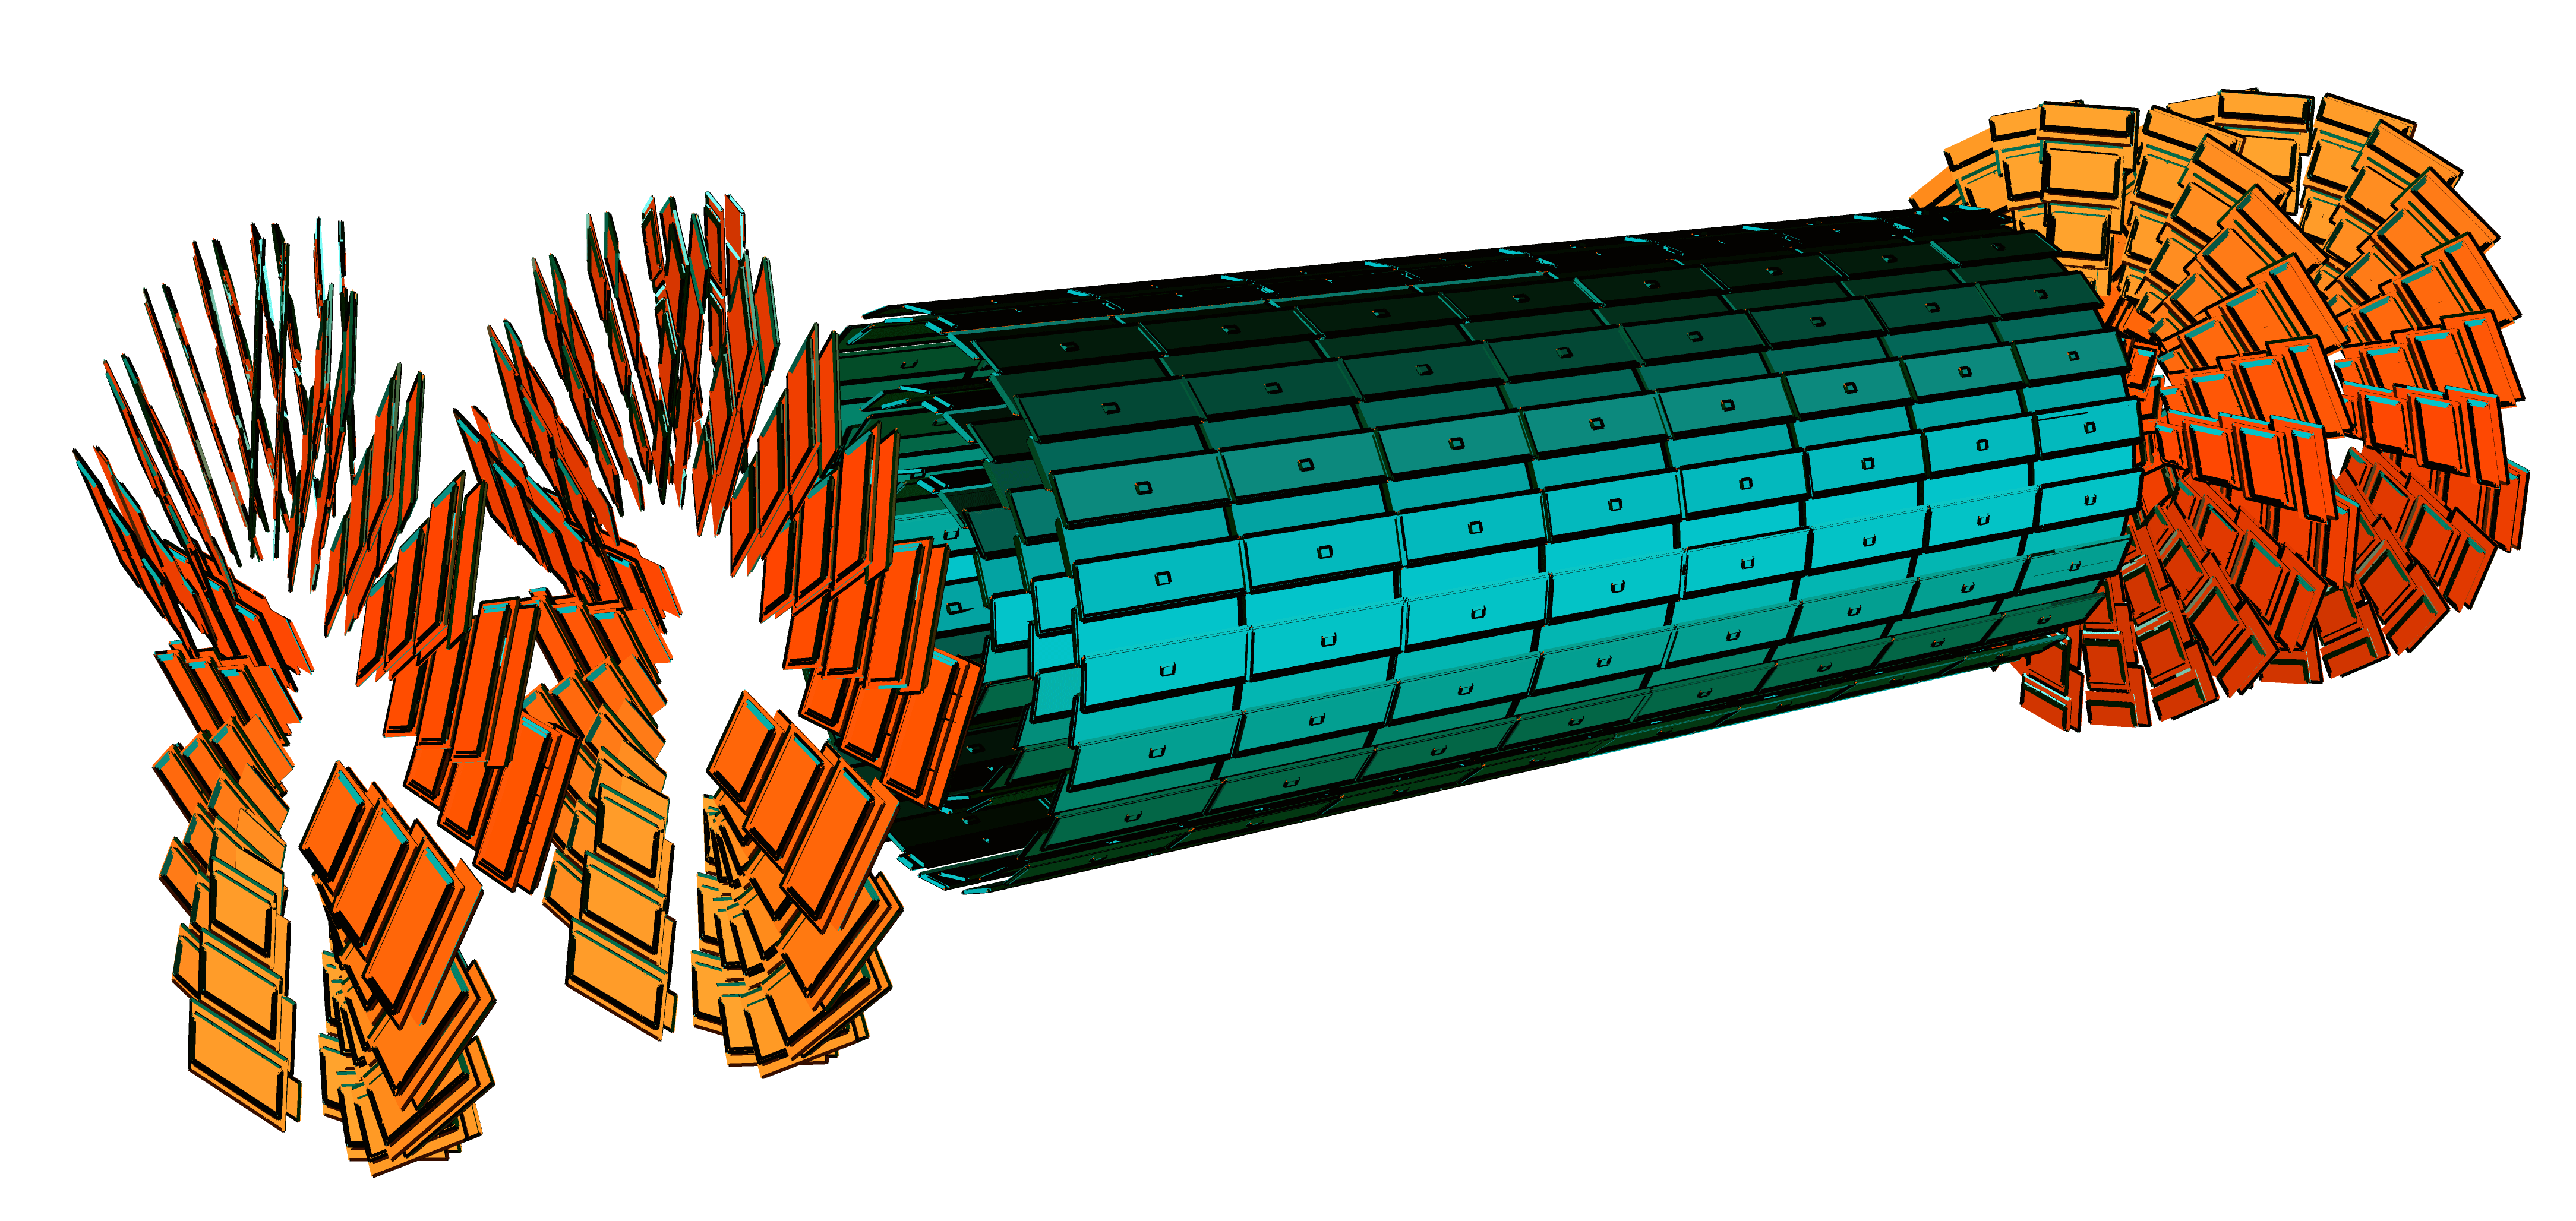
\includegraphics[width=8cm]{CMS_chapter_plots/pixel2} &
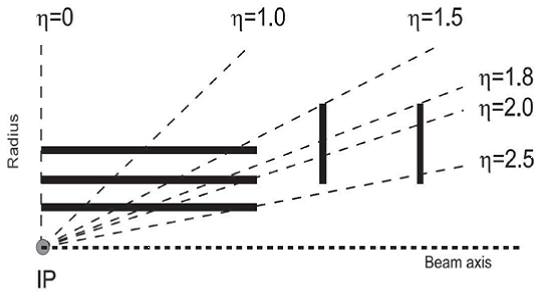
\includegraphics[width=8cm]{CMS_chapter_plots/pixel3}
\end{tabular}
  \caption*{Source: Commissioning and Performance of the CMS Pixel Tracker with Cosmic Ray Muons \cite{Chatrchyan:2009aa}, Radiation experience with the CMS pixel detector \cite{Veszpremi:2014exa}. }
\end{figure}

\subsubsection{Silicon Strips} \label{strip}

The Silicon Strip Tracker (SST) consists of four main subsystems, shown in \cref{fig:strip}: the four-layer Tracker Inner Barrel (TIB), the six-layer Tracker Outer Barrel (TOB) and, on each side of the barrel region, the three-disk Tracker Inner Disks (TID), and the nine-disk Tracker End Caps (TEC). Each TID disk is made of three rings of modules, while TEC disks have seven rings. The whole SST has a diameter of \unit[2.4]{m} and a length of \unit[5.5]{m}, being the largest silicon detector ever built with an active area of \unit[198]{m$^{2}$}. Its acceptance ranges over a region in pseudo-rapidity $\left| \eta\right|$ < 2.5. This component of the tracker consist of 15 148 detector modules and comprises 9.3 million detector channels. Each detector module consists of a carbon or graphite fibre frame, which supports the silicon sensor and the associated front-end readout electronics.
 
The physical principle behind the strip detector is the same than the pixel detector. As a charged particle crosses the detector, interact with the electrons from the material producing a small pulse of current during a very short time. This small amount of charge is amplified by the APV25 chips, resulting in "hits", which are used for the path reconstruction. The charge on each microstrip is read out and amplified by an Analogue Pipeline Voltage (APV25) chip. Four or six such chips are housed within a “hybrid”, which also contains electronics to monitor key sensor information, such as temperature, and provide timing information in order to match “hits” with collisions. 

\begin{figure}[H]
  \caption{Strip and pixel silicon detector. \label{fig:strip}}
  \centering
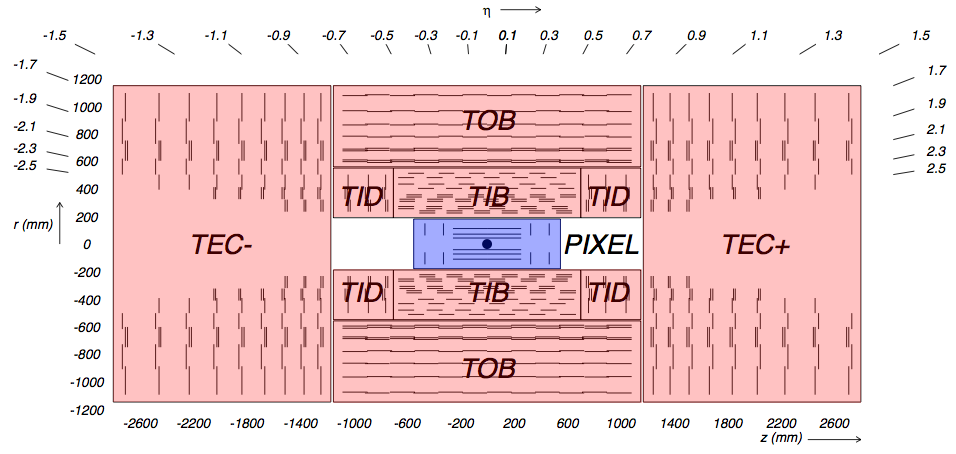
\includegraphics[width=10cm]{CMS_chapter_plots/strip}
  \caption*{Source: Description and performance of track and primary-vertex
                          reconstruction with the CMS tracker \cite{Chatrchyan:2014fea}.}
\end{figure}

\subsection{Electromagnetic Calorimeter (ECAL)}

The electromagnetic calorimeter of CMS (ECAL) is a hermetic homogeneous calorimeter. It is divided in three sections; a barrel section and two endcap sections. The barrel covers the pseudo-rapidity region $\eta$ < 1.48 and is constructed from 61200 lead tungstate crystals. The crystals are grouped into units, called supermodules, of 1700 crystals. There are 36 supermodules in the barrel. The endcaps cover the pseudo-rapidity region 1.48 < $\eta$ < 3.0. Each endcap is made from two ‘Dees’ and 7244 crystals. The crystals are grouped into modules of 25 crystals, known as supercrystals. The inner and outer boundaries of the endcaps are made more circular by the addition of smaller units known as partial supercrystals.

\begin{figure}[H]
  \caption{Electromagnetic Calorimeter \label{fig:caloc}}
  \centering
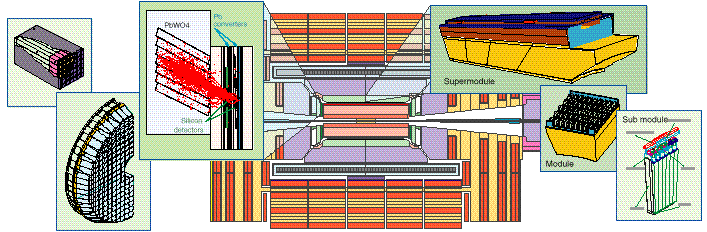
\includegraphics[width=14cm]{CMS_chapter_plots/caloc}
\end{figure}
\noindent
Lead tungstate (PbWO4) is a dense, fast and radiation-tolerant scintillating crystal. These three properties of the crystal make it an ideal choice for the CMS ECAL. The short radiation length and small Moliere radius allow a compact calorimeter to be constructed. The scintillation decay time is very fast with 80$\%$ of the scintillation light collected within 25ns (in the LHC bunches of protons collide every 25ns). 

\subsection{Hadronic Calorimeter (HCAL)}

The HCAL is a sampling calorimeter which determine the position, energy and arrival time of a particle using alternating	 layers of "absorber" and fluorescent "scintillator" materials that produce a rapid light pulse when the particle passes through. Special optic fibres collect up this light and deliver it into readout boxes where photodetectors amplify the signal. When the amount of light in a given region is summed up over many layers of tiles in depth, called a "tower", this total amount of light is a measure of a particle’s energy. 

The hadron calorimeter barrel is radially restricted between the outer extent of the electromagnetic calorimeter (R = 1.77 m) and the inner extent of the magnet coil (R = 2.95 m). This constrains the total amount of material which can be put in to absorb the hadronic shower. Therefore, an outer hadron calorimeter is placed outside the solenoid complementing the barrel calorimeter. Beyond $|\eta| = 3$, the forward hadron calorimeters placed at 11.2 m from the interaction point extend the pseudorapidity coverage down to $|\eta| = 5.2$. 

The HCAL is organized into barrel (formed by two sections : Hadron Barrel(HB) in the region $|\eta|$ < 1.4 and Hadron Outer (HO) in the region $|\eta|$ < 1.26), Hadron Endcap (HE) [1.3<$|\eta|$ < 3.0]  and Hadron Forward (HF) [2.9<$|\eta|$ < 5.0]  sections.(Fig. \ref{fig:hcal1})

\begin{figure}[H]
  \caption{Longitudinal view of the CMS detector showing the locations of the hadron barrel
  (HB), endcap (HE), outer (HO) and forward (HF) calorimeters. \label{fig:hcal1}}
  \centering
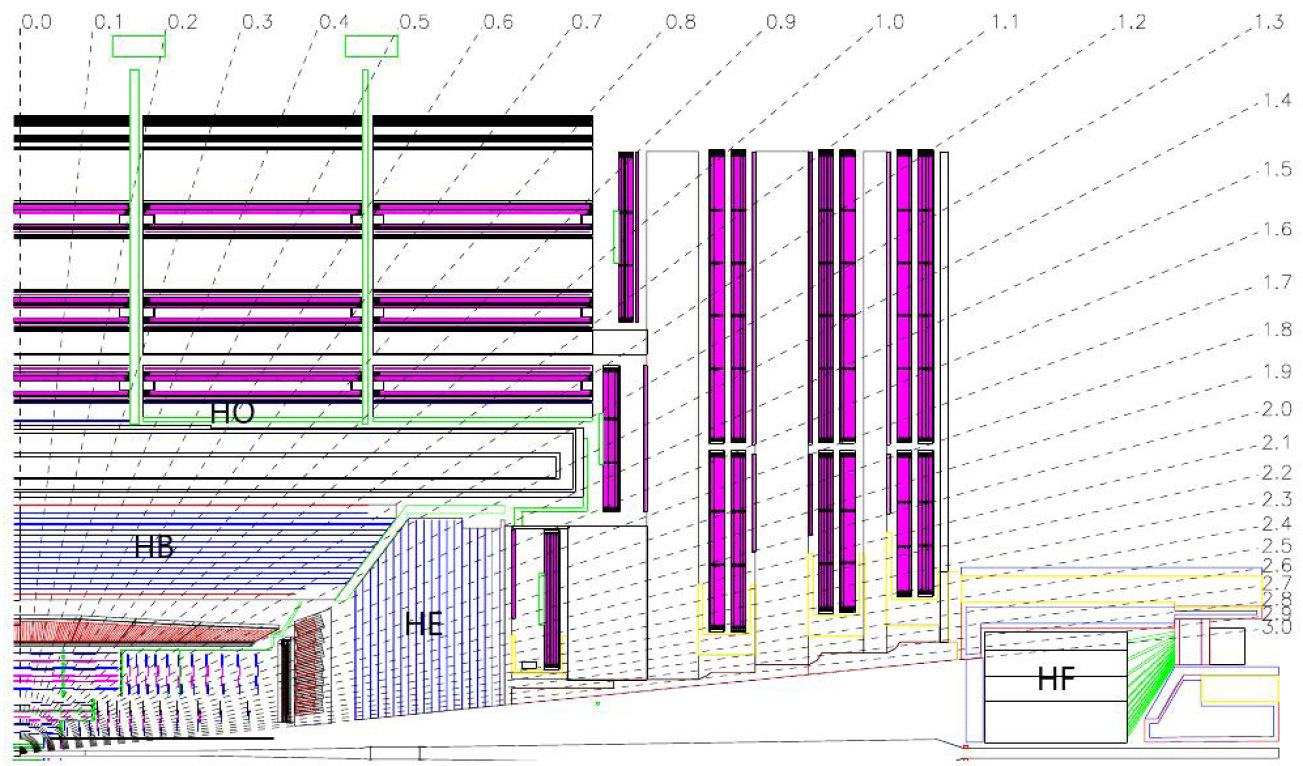
\includegraphics[width=9cm]{CMS_chapter_plots/hcal1}
\end{figure}

The HB is a sampling calorimeter covering the pseudorapidity range $|\eta|$ < 1.4, resulting in 2304 towers with a segmentation $\Delta\eta\times\Delta\phi=0.087\times 0.087$. The HB consists of 36 identical azimuthal wedges which form the two half-barrels (HB$+$ and HB$-$).

\begin{figure}[H]
  \caption{View of an HB wedge. \label{fig:hcal3}}
  \centering
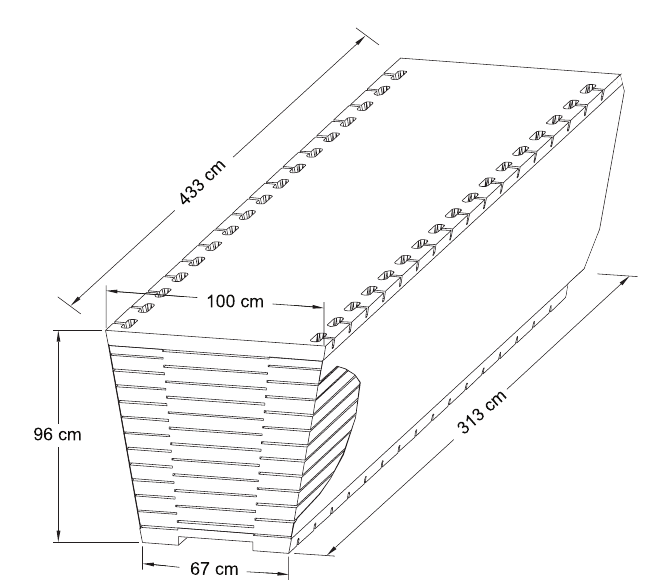
\includegraphics[width=8cm]{CMS_chapter_plots/hcal3}
\end{figure}

The wedges (Fig. \ref{fig:hcal3}) are constructed out of flat brass absorber plates aligned parallel to the beam axis.
The HB baseline active material is 3.7 mm thick Kuraray SCSN81 plastic scintillator, chosen for its long term stability and moderate radiation hardness. The granularity of the HCAL is 25 times coarser than that of
the ECAL, which would not allow charged and neutral hadrons to be spatially separated in jets with a transverse momentum much above 100 GeV/c. The hadron energy resolution in the combined ECAL-HCAL system is, however, of the order of 10$\%$ at 100 GeV. This resolution allows neutral hadrons to be detected as an energy excess on top of the energy deposited by the charged hadrons pointing to the same calorimeter cells. 

\subsection{The Muon System}

Muons are an unmistakable signature of most of the physics LHC is designed to explore. The ability to trigger on and reconstruct muons at the highest luminosities is central to the concept of CMS. Muons can penetrate several metres of iron without interacting. Unlike most particles they are not stopped by any of the calorimeter detectors ($\tau \approx$ 2.2 $\mu$s). Therefore, chambers to detect muons are placed at the very edge of the experiment where they are the only particles likely to register a signal. 

The CMS muon system is designed to have the capability of reconstructing the momentum and charge of muons over the the entire kinematic range of the LHC. The Muon system is a class of tracking detector, and is divided in two main regions: the Barrel ($|\eta|$< 1.2) and  the endcap (1.2 <$|\eta|$< 2.4). There are three types of detectors in the Muon System:

\paragraph{Drift Tubes (DT)}
The drift tube (DT) chamber (Fig. \ref{fig:DT}) system measures muon positions in the barrel part of the detector. The chamber volume is filled with a Ar(85 $\%$)/CO$_{2}$(15 $\%$) gas mixture, kept at atmospheric pressure.  When a muon or any charged particle passes through the volume, it knocks electrons off the atoms of the gas. By registering where along the wire electrons hit, as well as by calculating the muon's original distance away from the wire, DTs give two coordinates for the muon’s position.
\begin{figure}[H]
  \caption{Muon Drift Tubes \label{fig:DT}}
  \centering
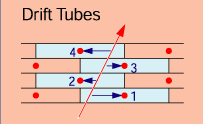
\includegraphics[width=6cm]{CMS_chapter_plots/DT}
\end{figure}
\paragraph{Cathode Strip Chamber (CSC)}
Cathode strip chambers (CSC) are used in the endcap disks where the magnetic field is inhomogeneous and particle rates are high. CSCs consist of arrays of positively charged "anode" wires crossed with negatively charged copper "cathode" strips within a gas volume. When muons pass through, they knock electrons off the gas atoms, which flock to the anode wires creating an avalanche of electrons. Positive ions move away from the wire and towards the copper cathode, also inducing a charge pulse in the strips, at right angles to the wire direction.
\begin{figure}[H]
  \caption{Cathode Strip Chamber \label{fig:CSC}}
  \centering
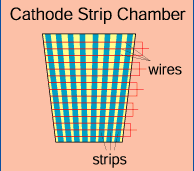
\includegraphics[width=5cm]{CMS_chapter_plots/CSC}
\end{figure}

\paragraph{Resistive Plate Chambers (RPC)}
Resistive plate chambers (RPC) are fast gaseous detectors that provide a muon trigger system parallel with those of the DTs and CSCs. RPCs consist of two parallel plates, a positively-charged anode and a negatively-charged cathode, both made of a very high resistivity plastic material and separated by a gas volume. When a muon passes through the chamber, electrons are knocked out of gas atoms. These electrons in turn hit other atoms causing an avalanche of electrons. The electrodes are transparent to the signal (the electrons), which are instead picked up by external metallic strips after a small but precise time delay. The pattern of hit strips gives a quick measure of the muon momentum, which is then used by the trigger to make immediate decisions about whether the data are worth keeping. RPCs combine a good spatial resolution with a time resolution of just one nanosecond (one billionth of a second).
\begin{figure}[H]
  \caption{Resistive Plate Chambers \label{fig:RPClayers}}
  \centering
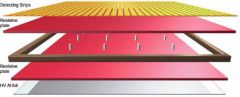
\includegraphics[width=5cm]{CMS_chapter_plots/RPClayers}
\end{figure}

In total there are 1400 muon chambers: 250 drift tubes (DTs) and 540 cathode strip chambers (CSCs) track the particles’ positions and provide a trigger, while 610 resistive plate chambers (RPCs) form a redundant trigger system, which quickly decides to keep the acquired muon data. The Barrel Detector consists of 4 concentric “stations” (Fig. \ref{fig:mustations}) of 250 chambers inside the magnet return yoke of CMS, which is in turn divided into 5 wheels. Each wheel is divided into 12 sectors, each covering a $30^{\circ}$ azimuthal angle. The 2 innermost stations, named MS1 and MS2, consist of “sandwiches” made of a DT chamber placed between 2 RPCs. The 2 outermost stations, MS3 and MS4, consist of packages of a DT chamber coupled to a layer made of 1, 2, or 4 RPCs, depending on the sector and station, placed on the innermost side of the station.

\begin{figure}[H]
  \caption{Muons Stations \label{fig:mustations}}
  \centering
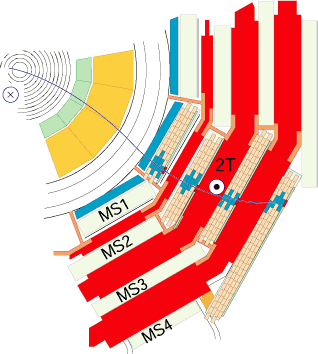
\includegraphics[width=6cm]{CMS_chapter_plots/mustations}
\end{figure}

\section{CMS Data Acquisition and Triggering}\label{triggerbase}

When CMS performs at its peak, about one billion proton-proton interactions will take place every second inside the detector. There is no way that data from all these events could be read out, and even if they could, most would be less likely to reveal new phenomena. We therefore need a "trigger" that can select the potentially interesting events, and reduce the rate to just a few hundred "events" per second, which can be read out and stored on computer disk for subsequent analysis. This task is performed by the trigger system, which is the start of the physics event selection process. The rate is reduced in two steps called Level-1 (L1) Trigger and High-Level Trigger (HLT), respectively. The Level-1 Trigger consists of custom-designed, largely programmable electronics, whereas the HLT is a software system implemented in a filter farm of about one thousand commercial processors. The rate reduction capability is designed to be at least a factor of $10^{6}$ for the combined L1 Trigger and HLT. 

Level 1 of the trigger is an extremely fast and wholly automatic process that looks for simple signs of interesting physics, e.g. particles with a large amount of energy or in unusual combinations. The Level 1 trigger select the best 100,000 events each second from the billion available. For the next test, the HLT assimilate and synchronise information from different parts of the detector to recreate the entire event and send it to a farm of more than 1000 standard computers.

\begin{figure}[H]
  \caption{CMS Triggering System \label{fig:TRIGGER}}
  \centering
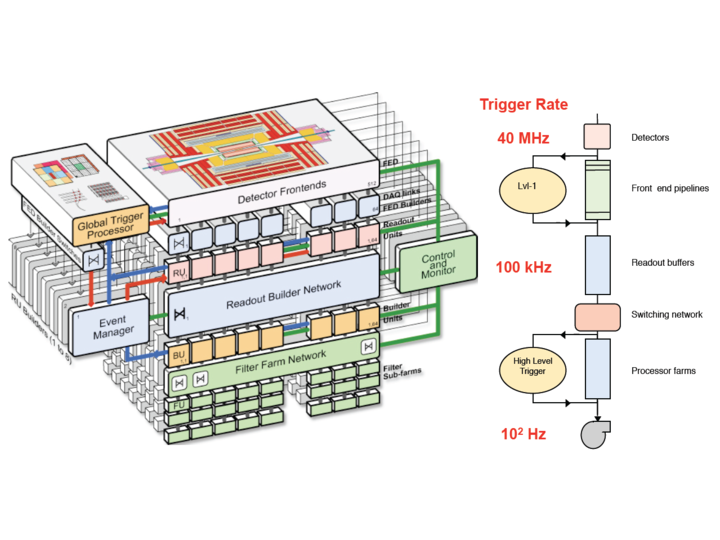
\includegraphics[width=14cm]{CMS_chapter_plots/TRIGGER}
\end{figure}

\begin{comment}
\subsection{Luminosity}
In particle physics experiments the energy available for the production of new effects is the most im-
portant parameter. The required large centre of mass energy can only be provided with colliding beams
where little or no energy is lost in the motion of the centre of mass system (cms). Besides the energy the
number of useful interactions (events), is important. This is especially true when rare events with a small
production cross section sigmap are studied. The quantity that measures the ability of a particle accelerator
to produce the required number of interactions is called the luminosity and is the proportionality factor
between the number of events per second dR/dt and the cross section sigmap :
\end{comment}